\documentclass[UTF8]{ctexart}

\usepackage{fancyhdr}
\usepackage{titlesec}
\usepackage{geometry}
\geometry{a4paper,left=2cm,right=2cm,bottom=2.5cm,top=2.5cm}
\usepackage{graphicx}
\usepackage{epstopdf}
\usepackage{ctexbook}
\usepackage{ctexrep}
\usepackage{listings}
\usepackage{indentfirst}
\graphicspath{ {figure/} } 

\pagestyle{fancy}
\lhead{} 
\chead{\bfseries 光信息科学与技术实验} 
\rhead{} 
\lfoot{} 
\cfoot{\thepage}
\rfoot{} 
\renewcommand{\headrulewidth}{0.4pt} 
\renewcommand{\footrulewidth}{0.4pt}

\newcommand{\major}{计算机应用技术,精密仪器及机械}
\newcommand{\name}{杜沈达,王晨}
\newcommand{\stuid}{SA18168163,SA18168095}
\newcommand{\newdate}{\today}
\newcommand{\loc}{物理楼}
\newcommand{\course}{光信息科学与技术实验}
\newcommand{\grades}{}
\newcommand{\newtitle}{利用DOE对光场进行整形变换}

\makeatletter
\newcommand{\figcaption}{\def\@captype{figure}\caption}
\newcommand{\tabcaption}{\def\@captype{table}\caption}
\makeatother
\setlength{\parindent}{2.45em}

\begin{document}
\thispagestyle{empty}
	\begin{figure}[h]
		\begin{minipage}{0.6\linewidth}
			
\includegraphics[width=\linewidth]{head.jpg}
		\end{minipage}
		\hfill
		\begin{minipage}{.4\linewidth}
			\raggedleft
			\begin{tabular*}{.8\linewidth}{ll}
				专业: & \underline\major   \\
				姓名: & \underline\name    \\
				学号: & \underline\stuid   \\
				日期: & \underline\newdate \\
				地点: & \underline\loc
			\end{tabular*}
		\end{minipage}
	\end{figure}
	
	\begin{table}[!htbp]
		\centering
		\begin{tabular*}{\linewidth}{llllll}
			课程名称: & \underline\course   & 
			实验名称: & \underline\newtitle & 
			成绩:     & \underline\grades \\
		\end{tabular*}
	\end{table}

\titleformat*{\section}{\large\bfseries}
\titleformat*{\subsection}{\normalsize\bfseries}
\titleformat*{\subsubsection}{\normalsize}

\section{实验原理和目的}
	\subsection{实验原理}

DOE是Diffractive Optical Elements的缩写,中文翻译是衍射光学元件。这是利用光波的衍射理论,利用计算机辅助设计,超大规模集成(VLSI)电路制造工艺,在偏基上刻蚀产生台阶或连续浮雕结构,形成纯位相、同轴再现、具有极高衍射效率的一类衍射光学元件。实验原理如图1所示。
	\begin{center}
		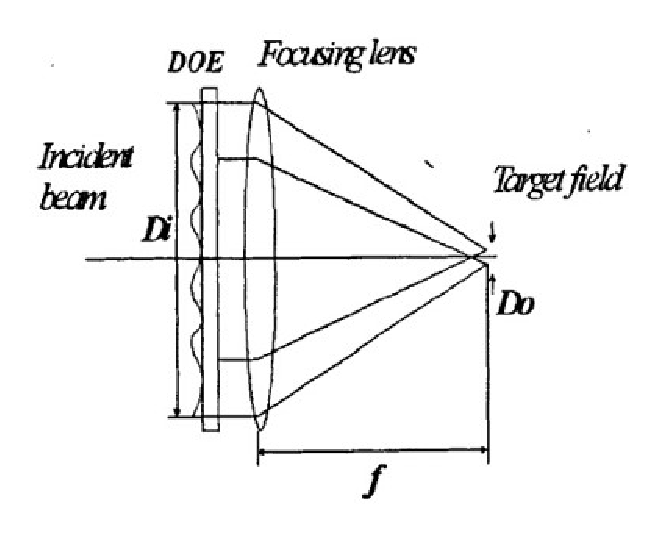
\includegraphics[width=7.5cm,height=5cm]{Prin.eps}
		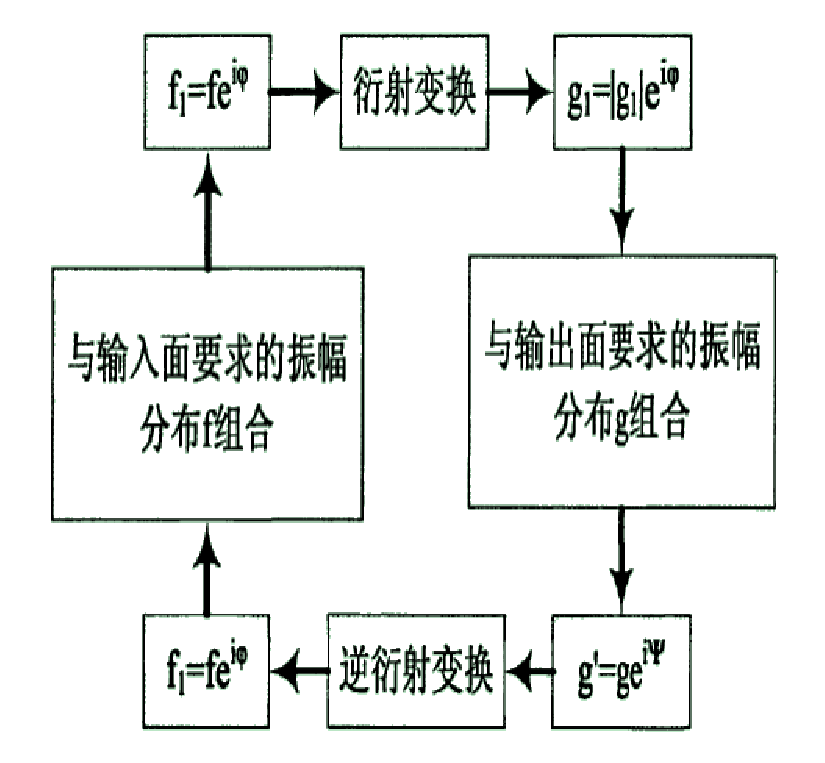
\includegraphics[width=7.5cm,height=5cm]{Desi.eps}
		\figcaption{实验原理和DOE设计}\label{Princeple}
	\end{center}
	
光从激光器出来,如果没有DOE,那么它通过透镜就聚焦于一点,产生原来的性质,现在加了DOE光就经过调制,改变了原来的光了,通过设计DOE的形状,也就可以产生不同的光路,从而得到想要的光场。也就是从高斯光强分布到矩形均匀光强分布。从左图可以看出,经过调制的光再经过透镜也有一个目标域,这也就是说调制后的光经过透镜依旧会有一个最好的成像距离,在后面的实验中,我们也在改变CCD在光轴上的距离来观察这个最好成像距离的位置和透镜焦距的关系。
	
如图2所示,DOE整形分系统由一片透射式位相型DOE和一片紧密连接的Fourier透镜组成,这种结构在DOE设计中属于1f 工作方式整形器。1f 结构的工作装置中,DOE 将输入光场的位相及振幅进行调制,利用透镜使出射光束在成像面叠加。这种结构对DOE
的设计质量要求较高,但透镜只是起到聚焦作用,所以,整个工作装置的尺寸自由度较高,同时对光场整形的效果也完全取决于DOE,只需要根据成像距离调节适应的透镜焦距就可以很好地起到光场内的衍射光位相叠加。
\begin{center}
	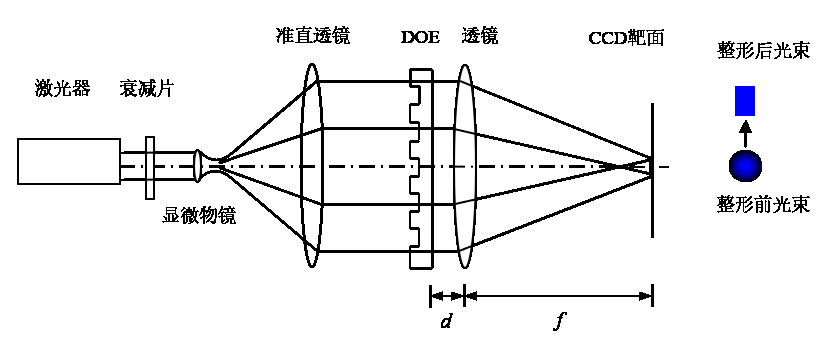
\includegraphics{Proc.eps}
	\figcaption{DOE整形系统原理示意图}
\end{center}
	\subsection{实验过程}
	\begin{enumerate}
\item 参照图2搭建实验平台,首先由He-Ne激光器产生一束激光,在光路中先加准直透镜,观察激光在墙上的位置并且记录。之后再加透镜并且不断调整,使得两次激光的光点在同一位置。这就保证了光路同轴条件;
\item 开启激光器,选用合适衰减片至光强合适,打开CCD及数采监控计算机系统,观察图像,通过调整CCD前后位置使图像清晰,以达到CCD探头平面与透镜焦平面重合;
\item 观察没有DOE情况下,焦平面高斯光强分布。并采集一幅图像保存;
\item 将DOE放入光路中,调节其中心与透镜中心同轴及其平面与光轴垂直;
\item 观察此时的图像、光强分布。再采集一副图像保存;
\item 移动DOE偏离光轴,观察图像的光强分布,并保存;	
\item 实验结束,关闭激光器,CCD,计算机,整理平台,把实验器件归位。
	\end{enumerate}
	\subsection{实验目的}	
	\begin{enumerate}
	\item 了解使用 DOE 对光束实现整形变换的意义及原理 
	\item 熟悉光场测试的基本过程,学习 CCD 的使用 
	\item 观测各个光学元器件表面反射和干涉对测试结果的影响 
	\end{enumerate}

\section{实验结果}
	\subsection{实验结果处理过程}
我们在经过实验后,得到了一幅在DOE调制光场前的激光图片,五幅各个角度的图片和五幅从CCD与DOE相距25cm~29cm的图。共十一幅图片,使用实验计算机截图CCD捕捉到的图片,再用MATLAB软件进行光强分析,观察DOE调制前后的是否有差别,旋转衰减片产生的影响和移动CCD是否会因为和DOE之间的距离而有变化。
	\subsection{实验结果图}
		\begin{center}
			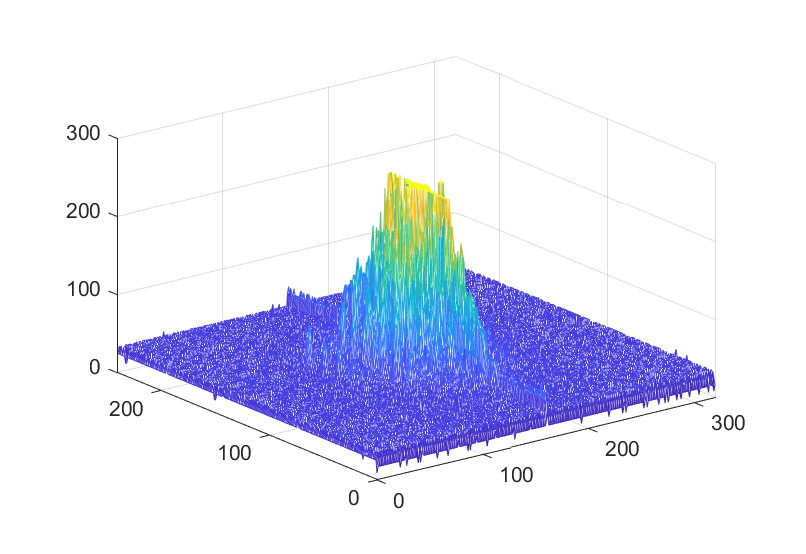
\includegraphics[width=15cm,height=10cm]{d3.eps}
			\figcaption{未加DOE的xy平面的亮度图}
			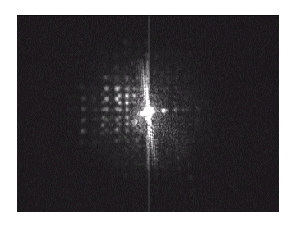
\includegraphics[width=7.5cm,height=7.5cm]{YUANbeforeDOE.eps}
			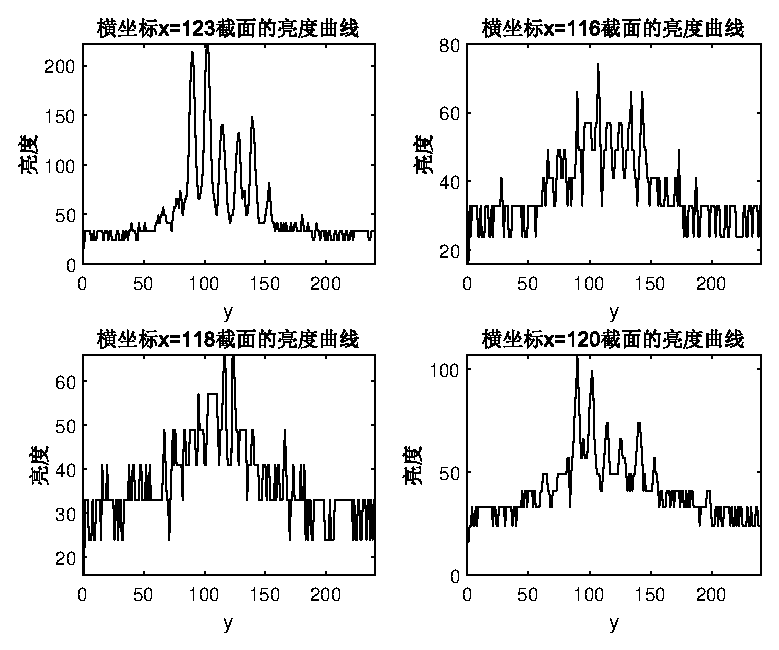
\includegraphics[width=7.5cm,height=7.5cm]{beforeDOE.eps}
			\figcaption{未加DOE的CCD捕捉图和光亮度曲线}\label{beforeDOE}
			
			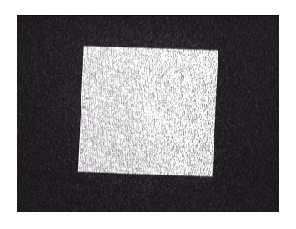
\includegraphics[width=7.5cm,height=7.5cm]{YUANaddDOEangel1.eps}
			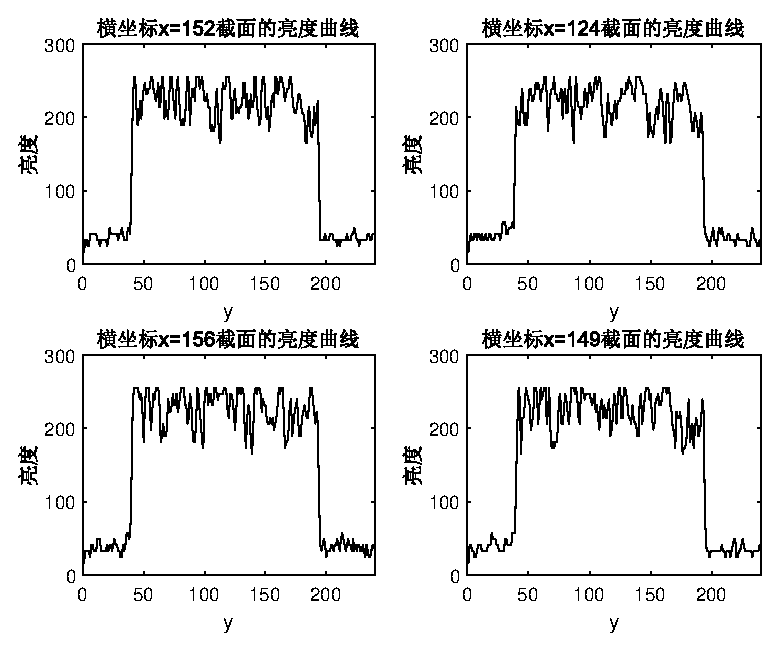
\includegraphics[width=7.5cm,height=7.5cm]{addDOEangel1.eps}
			\figcaption{加DOE的CCD捕捉图和光亮度曲线(角度1)}\label{addDOEangel1}
			
			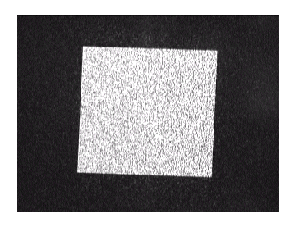
\includegraphics[width=7.5cm,height=7.5cm]{YUANaddDOEangel2.eps}
			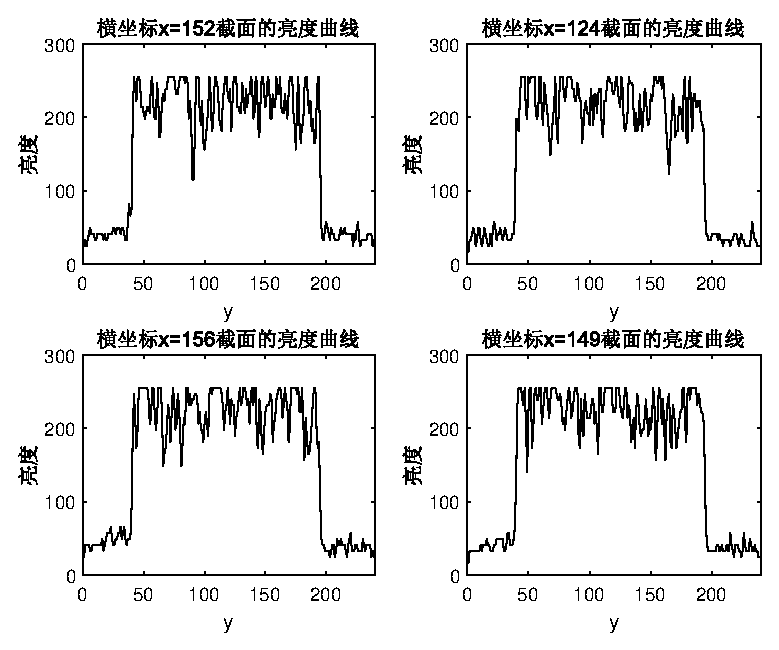
\includegraphics[width=7.5cm,height=7.5cm]{addDOEangel2.eps}
			\figcaption{加DOE的CCD捕捉图和光亮度曲线(角度2)}\label{addDOEangel2}
			
			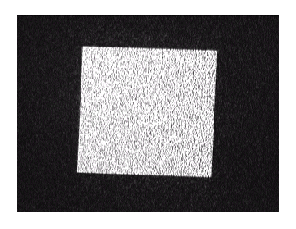
\includegraphics[width=7.5cm,height=7.5cm]{YUANaddDOEangel3.eps}
			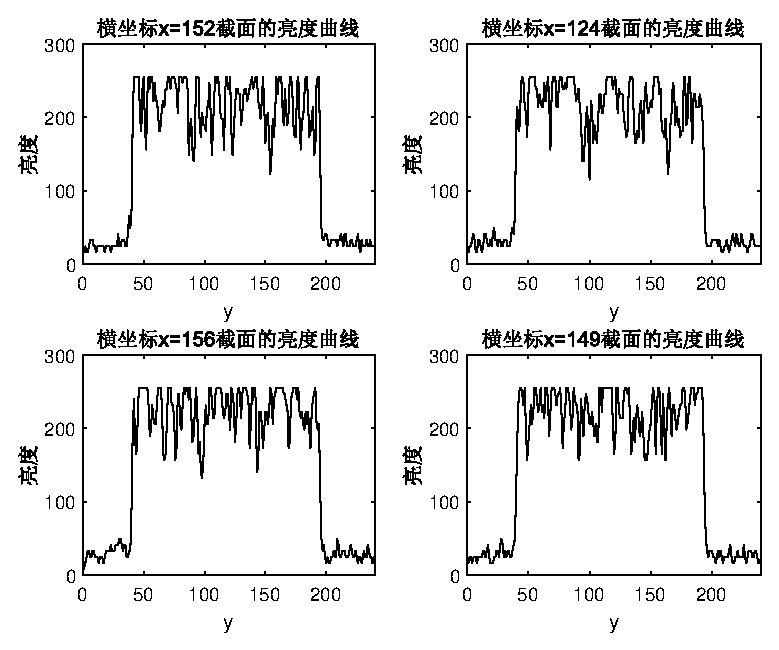
\includegraphics[width=7.5cm,height=7.5cm]{addDOEangel3.eps}
			\figcaption{加DOE的CCD捕捉图和光亮度曲线(角度3)}\label{addDOEangel3}
			
			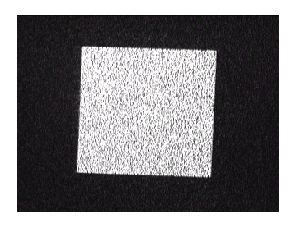
\includegraphics[width=7.5cm,height=7.5cm]{YUANaddDOEangel4.eps}
			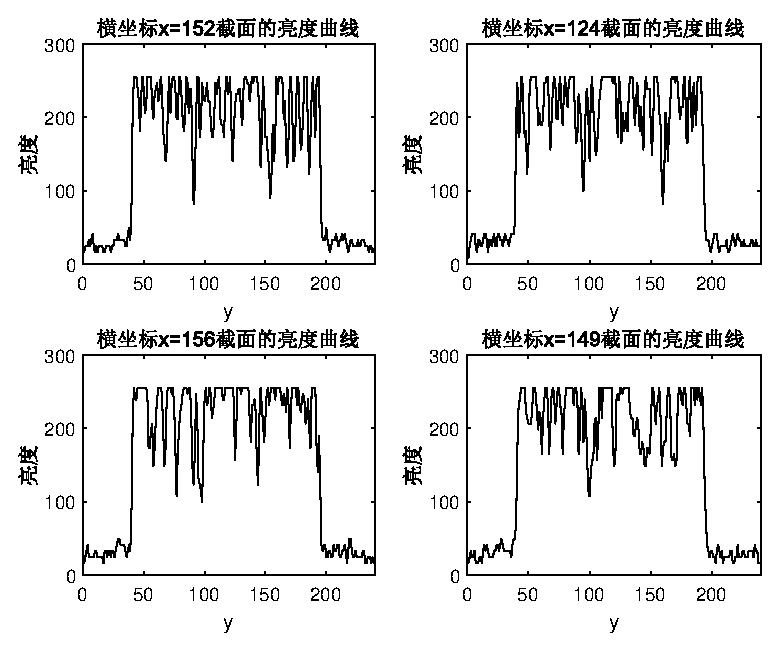
\includegraphics[width=7.5cm,height=7.5cm]{addDOEangel4.eps}
			\figcaption{加DOE的CCD捕捉图和光亮度曲线(角度4)}\label{addDOEangel4}
			
			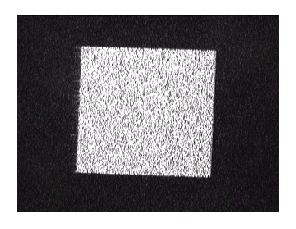
\includegraphics[width=7.5cm,height=7.5cm]{YUANaddDOEangel5.eps}
			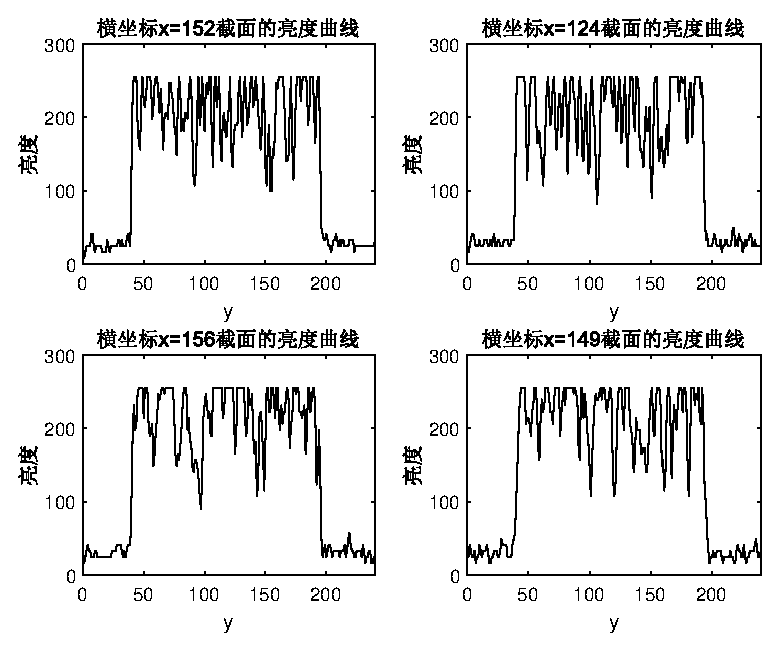
\includegraphics[width=7.5cm,height=7.5cm]{addDOEangel5.eps}
			\figcaption{加DOE的CCD捕捉图和光亮度曲线(角度5)}\label{addDOEangel5}
			
			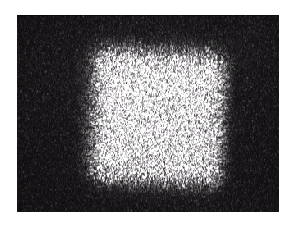
\includegraphics[width=7.5cm,height=7.5cm]{YUANaddDOEmoveCCD25.eps}
			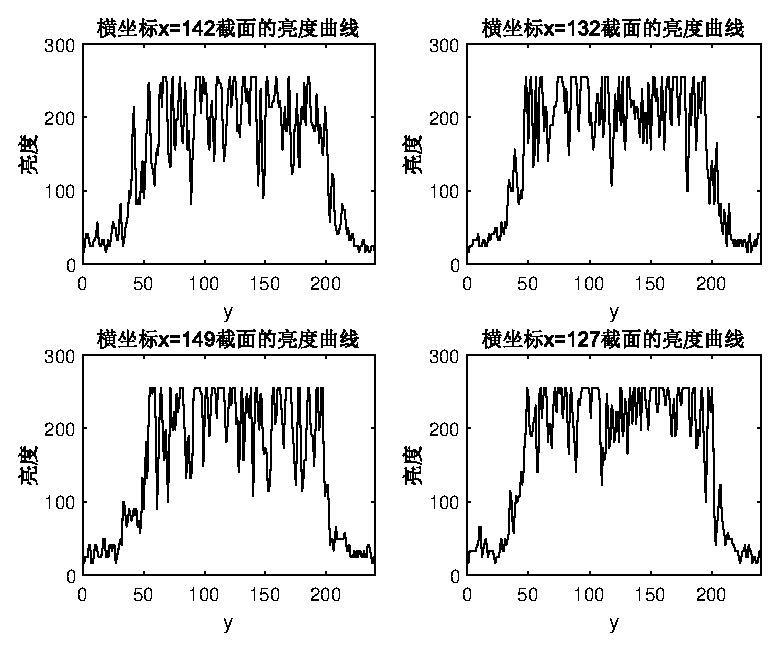
\includegraphics[width=7.5cm,height=7.5cm]{addDOEmoveCCD25.eps}
			\figcaption{加DOE的CCD捕捉图和光亮度曲线(CCD与DOE距离25cm)}\label{addDOEmoveCCD25}
			
			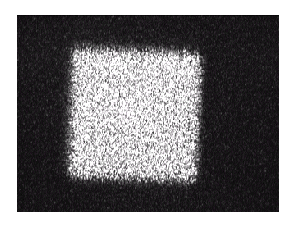
\includegraphics[width=7.5cm,height=7.5cm]{YUANaddDOEmoveCCD26.eps}
			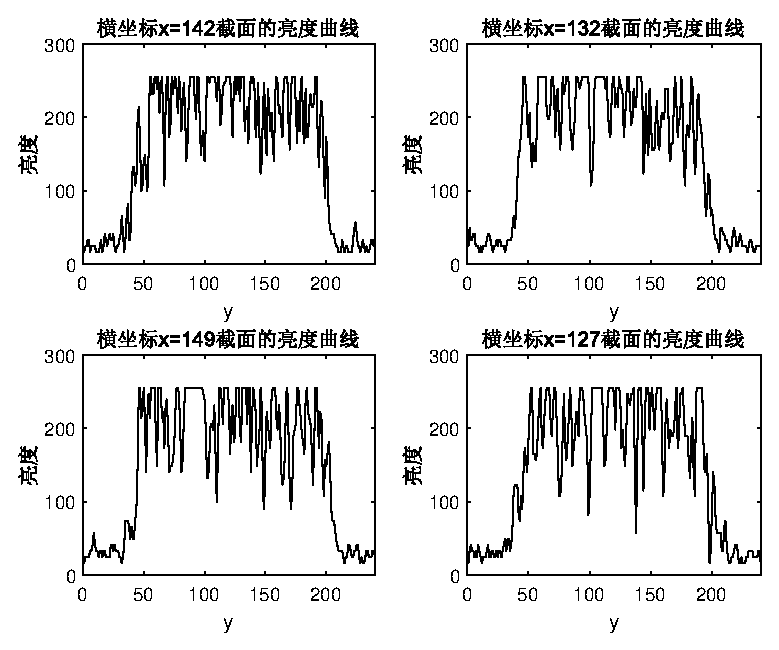
\includegraphics[width=7.5cm,height=7.5cm]{addDOEmoveCCD26.eps}
			\figcaption{加DOE的CCD捕捉图和光亮度曲线(CCD与DOE距离26cm)}\label{addDOEmoveCCD26}
			
			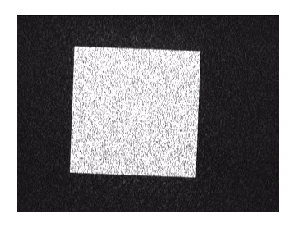
\includegraphics[width=7.5cm,height=7.5cm]{YUANaddDOEmoveCCD27.eps}
			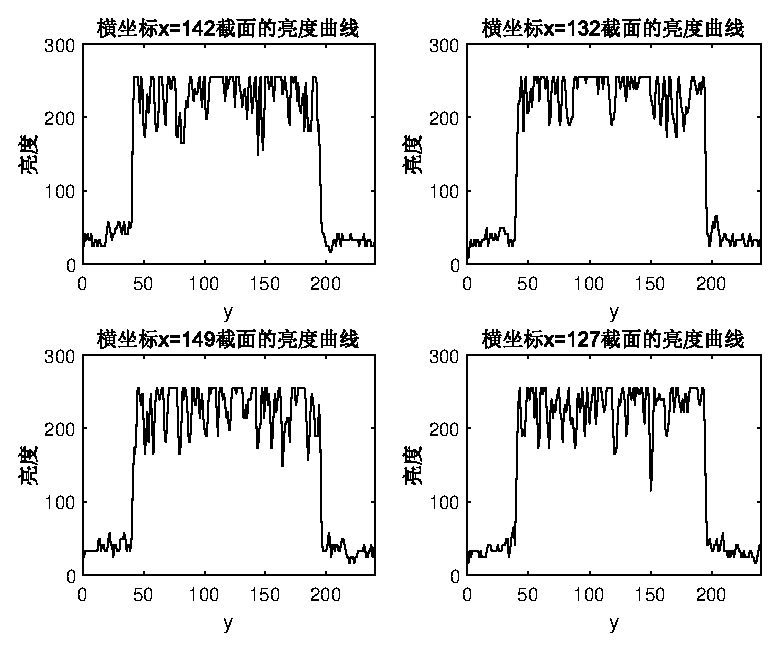
\includegraphics[width=7.5cm,height=7.5cm]{addDOEmoveCCD27.eps}
			\figcaption{加DOE的CCD捕捉图和光亮度曲线(CCD与DOE距离27cm)}\label{addDOEmoveCCD27}
			
			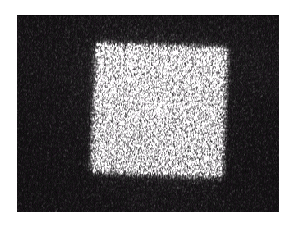
\includegraphics[width=7.5cm,height=7.5cm]{YUANaddDOEmoveCCD28.eps}
			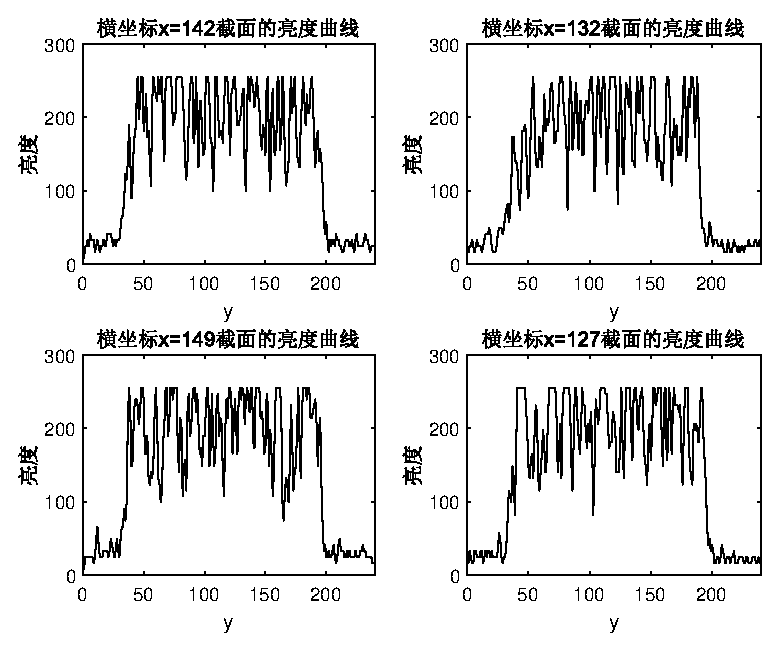
\includegraphics[width=7.5cm,height=7.5cm]{addDOEmoveCCD28.eps}
			\figcaption{加DOE的CCD捕捉图和光亮度曲线(CCD与DOE距离28cm)}\label{addDOEmoveCCD28}
			
			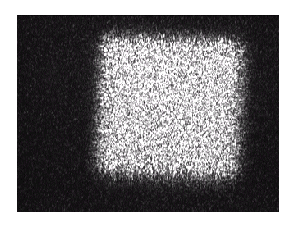
\includegraphics[width=7.5cm,height=7.5cm]{YUANaddDOEmoveCCD29.eps}
			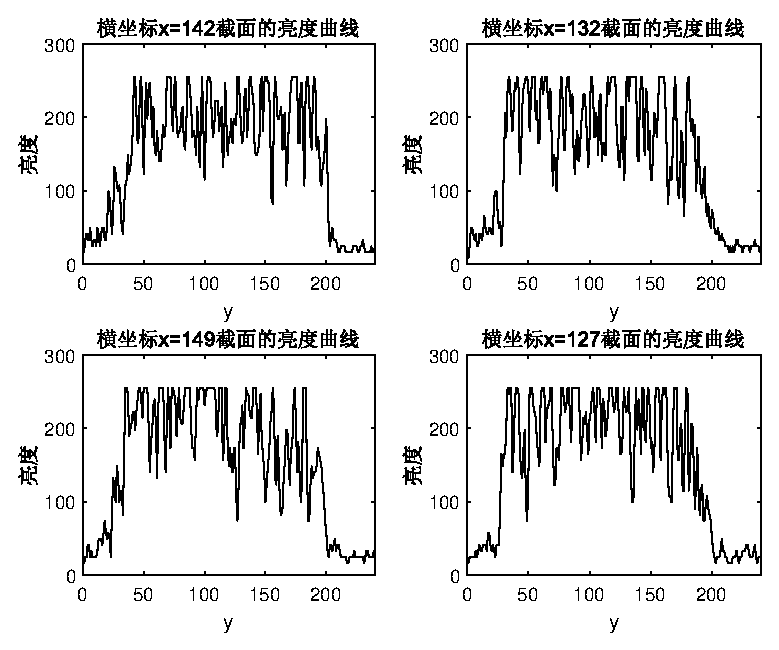
\includegraphics[width=7.5cm,height=7.5cm]{addDOEmoveCCD29.eps}
			\figcaption{加DOE的CCD捕捉图和光亮度曲线(CCD与DOE距离29cm)}\label{addDOEmoveCCD29}
		\end{center}
	\subsection{实验结果分析}	
可以看到,实验得到的图像在未加DOE进行光场调制前是一个类似光强高斯分布的椭圆,也符合常理。在图像中看到的周围的白点,是由于在搭建光路的时候,各个光学元器件并没有百分百同轴,部分激光在光路中不断反射衍射产生的。
	
之后我们固定CCD等元件,只转动减振片,如图5~9所示,转动的方向是从上往下看逆时针,角度不断增大,截取五个角度点用CCD捕捉DOE调制后的光场图,并且画出其光强曲线。可以从CCD捕捉的图看出,从一开始到不断旋转衰减片,图片中白色矩形部分的黑点在增加,这也就是说明了DOE的调制跟激光射入的角度有关。

在只移动DOE在光轴上的位置的时候,可以发现27cm处的光场最为清晰明亮,从光强分布图上看,这个产生的平面上的光强相较于其他四幅图在矩形处的光强变化的差值也最小。
	
从输出结果图可以看出,整形光场顶部平滑,边缘轮廓清晰明显,中间附近产生的尖锐性突起是反射产生的,总体来说整形光场的均匀度好,能量转换效果也很好
	\subsection{实验代码}
实验代码大体上如下,使用一个循环读入图片再输出。值得说明的是,在选取x截面的时候,因为我们的图片并不是长宽水平与竖直的,所以选择边缘点的危险,所以我们限制了x的选取范围,也就是去除了可能取到边缘点影响结果的点。之后使用一串随机数产生四个随机的x的值,画出分别对应该x的y与光强的曲线图。当然,代码处理图片的前提是需要命名好图片的名称,再统一打印出来。在第2行中设置x取值的边界这么小的原因是我们在做实验的时候不能精确的移动CCD,造成了几幅图像的边界有偏移,而且矩形的边也不是完全水平和竖直的,所以取得边界会比实际矩形的边界要小。
	
处理五个旋转图片的代码如下:
		\lstinputlisting[language={MATLAB},
		numbers=left, numberstyle={\normalsize },	commentstyle=\color{red!50!green!50!blue!50}, 
		frame=shadowbox, rulesepcolor=\color{red!20!green!20!blue!20}]
		{code/angel.m}
	
对于五个改变距离的图片,只需要修改读入读出的语句即可,即改变代码块中的第5,第13和第16行为下述即可:
		\lstinputlisting[language={MATLAB},
		numbers=left, numberstyle={\normalsize },	commentstyle=\color{red!50!green!50!blue!50}, 
		frame=shadowbox, rulesepcolor=\color{red!20!green!20!blue!20}]
		{code/move.m}
\section{ 思考题与讨论}
	\begin{enumerate}
	
\item 实验中的噪声来源,如何避免及降低噪声对实验的影响?
实验中的噪声来源:
		\begin{enumerate}
\item 来自于光路中的元器件未同轴造成的,从未加DOE的图4CCD采集的照片来看,可以看到由于光路不同轴造成噪声在亮点周围的分布情况;
\item 于做实验时候外界的光造成影响,虽然把实验室的灯关了,但是由于电脑主机箱和显示屏的光依旧可能会对CCD采集造成一定的影响;
\item  光学膜片表面受到污染,需要清理。
		\end{enumerate}
解决方案:
		\begin{enumerate}
\item 在实验搭建光路的时候,应该保证光学元件的同轴度,也就是在搭好之后用CCD采集验证看其是否同轴;
\item 减少外界的光照,外界的光照会影响实验结果,最好是在无外界干扰光的情况下进行实验;
\item 实验前测试检验光学器件的镜片是否受到污染。
		\end{enumerate}

\item 有哪些方法可以提高光束整形的质量?
	\begin{enumerate}
\item 激光质量方面
		\begin{enumerate}
			\item  光斑椭圆,将其调整成规整的圆
			\item  在激光晶体棒套两端安装适当孔径的小孔光阑,这样激光输出能量会有所下降,但光束质量会得到改善。
		\end{enumerate}
\item  器件质量,光斑内部有明显缺陷,则光学膜片表面受到污染,需要清理。
\item 操作规范,保证光路同轴。

	\end{enumerate}
	\end{enumerate}

\section{本实验的收获,体会和建议}
经过本次实验,我们知道了为什么要进行光束整形,随着激光工程应用在越来越多的领域,需要激光能够适应不同的工程需求,对激光束进行整形的研究也越来越多。比如可以通过光场整形采用光镊技术来测量红细胞的弹性模量,将光束整形技术运用到医学影像领域等等。还知道通过DOE光场整形技术,可以把激光整形成任意形状的2D图形,甚至可以通过其他光场整形技术产生更为复杂的光场。通过实验,我们还学会怎样判断光路同轴的方法和利用DOE进行光场调制方法。
	
随着学习的深入,发现有那么多的新技术和看似不可思议的事情是在理论上是怎么验证,在实际中应该怎么做来实现的。也可以发现技术与科学的进步是相辅相成的,科学的交叉也越来越多,各个学课之间共同发展进步是未来的趋势。
	
\end{document}